\documentclass[a4j]{jsarticle}
\usepackage[dvipdfmx]{graphicx}
\usepackage{subcaption}
\usepackage{here}
\usepackage{listings}
\usepackage{ulem}
\usepackage{ascmac}
\usepackage{comment}
\usepackage[top=1.5cm, bottom=2cm, left=1.5cm, right=1.5cm]{geometry}



\title{回路システム基礎期末レポート}
\author{2231009 伊藤 大地}

\begin{document}
\maketitle
1ビットADコンバータのシミュレーションを行った.
入力信号には1Hzの正弦波を用いており,サンプリング周波数1kHzでオーバーサンプリングした.
図\ref{int}に入力信号の時間波形(1Hzの正弦波),図\ref{ins}に入力信号のスペクトル分布,図\ref{insk}に図\ref{ins}の低域部分を拡大したグラフを示す.

\begin{figure}[H]
 \centering
 \vspace{-3.5cm}
 \hspace{-2cm}
 \includegraphics[angle=-90,scale=0.6]{Input_time.eps}
 \vspace{-2cm}
 \caption{入力信号の時間波形(1Hzの正弦波)}
 \label{int}
\end{figure}

\begin{figure}[H]
 \centering
 \vspace{-4cm}
 \hspace{-2cm}
 \includegraphics[angle=-90,scale=0.6]{Input_spec.eps}
  \vspace{-2cm}
 \caption{入力信号のスペクトル分布}
 \label{ins}
\end{figure}

\begin{figure}[H]
 \centering
 \vspace{-4cm}
 \hspace{-2cm}
 \includegraphics[angle=-90,scale=0.6]{Input_spec_kakudai.eps}
  \vspace{-2cm}
 \caption{図\ref{ins}の低域部分を拡大したグラフ}
 \label{insk}
\end{figure}

%%%
\section*{(1) Plot output signals and spectrums 1st and 2nd $\Delta\Sigma$ modulators.}
%
\subsection*{(i) 1st $\Delta\Sigma$ modulators}
入力信号に1次$\Delta\Sigma$変調を行った結果を以下の図\ref{1stt}〜図\ref{1stsk}に示す.
図\ref{1stt}は1次$\Delta\Sigma$変調信号の時間波形,図\ref{1sts}はその信号のスペクトル分布,図\ref{1stsk}の低域部分を拡大したグラフである.

\begin{figure}[H]
 \centering
 \vspace{-3.5cm}
 \hspace{-2cm}
 \includegraphics[angle=-90,scale=0.6]{1stout_time.eps}
 \vspace{-2cm}
 \caption{1次$\Delta\Sigma$変調信号の時間波形}
 \label{1stt}
\end{figure}

\begin{figure}[H]
 \centering
 \vspace{-4cm}
 \hspace{-2cm}
 \includegraphics[angle=-90,scale=0.6]{1stout_spec.eps}
  \vspace{-2cm}
 \caption{1次$\Delta\Sigma$変調信号のスペクトル分布}
 \label{1sts}
\end{figure}

\begin{figure}[H]
 \centering
 \vspace{-4cm}
 \hspace{-2cm}
 \includegraphics[angle=-90,scale=0.6]{1stout_spec_kakudai.eps}
  \vspace{-2cm}
 \caption{図\ref{1sts}の低域部分を拡大したグラフ}
 \label{1stsk}
\end{figure}

%
\subsection*{(ii) 2nd $\Delta\Sigma$ modulators}
入力信号に2次$\Delta\Sigma$変調を行った結果を以下の図\ref{2ndt}〜図\ref{2ndsk}に示す.
図\ref{2ndt}は2次$\Delta\Sigma$変調信号の時間波形,図\ref{2nds}はその信号のスペクトル分布,図\ref{2ndsk}は図\ref{2nds}の低域部分を拡大したグラフである.

\begin{figure}[H]
 \centering
 \vspace{-3.5cm}
 \hspace{-2cm}
 \includegraphics[angle=-90,scale=0.6]{2ndout_time.eps}
 \vspace{-2.2cm}
 \caption{2次$\Delta\Sigma$信号の時間波形}
 \label{2ndt}
\end{figure}
\vspace{-5mm}

\begin{figure}[H]
 \centering
 \vspace{-4cm}
 \hspace{-2cm}
 \includegraphics[angle=-90,scale=0.6]{2ndout_spec.eps}
  \vspace{-2.2cm}
 \caption{2次$\Delta\Sigma$信号のスペクトル分布}
 \label{2nds}
\end{figure}
\vspace{-5mm}
\begin{figure}[H]
 \centering
 \vspace{-4cm}
 \hspace{-2cm}
 \includegraphics[angle=-90,scale=0.6]{2ndout_spec_kakudai.eps}
  \vspace{-2.2cm}
 \caption{図\ref{2nds}の低域部分を拡大したグラフ}
 \label{2ndsk}
\end{figure}
\vspace{-5mm}
%%%
\section*{(2) Plot the low-pass filtered signals of each output.}
ローパスフィルタとして1次のバタワースフィルタを用いた.また,カットオフ周波数は5Hzに設定した.以下の図\ref{lpf}にその周波数特性を示す.
\begin{figure}[H]
 \centering
 \vspace{-1cm}
 \hspace{-1cm}
 \includegraphics[angle=-90,scale=0.33]{H_spec.eps}
 \caption{1次バタワース型ローパスフィルタの周波数特性}
 \label{lpf}
\end{figure}
\vspace{-1cm}
%
\subsection*{(i) 1st $\Delta\Sigma$ modulators}
1次$\Delta\Sigma$変調信号に図\ref{lpf}のローパスフィルタを適用した結果を以下の図\ref{1lpft}〜図\ref{1lpfsk}に示す.
図\ref{1lpft}はローパスフィルタを適用した1次$\Delta\Sigma$変調信号の時間波形,図\ref{1lpfs}はその信号のスペクトル分布,図\ref{1lpfsk}は図\ref{1lpfs}の低域部分を拡大したグラフである.
\begin{figure}[H]
 \centering
 \vspace{-3.5cm}
 \hspace{-2cm}
 \includegraphics[angle=-90,scale=0.6]{1stout_LPF_time.eps}
 \vspace{-2cm}
 \caption{ローパスフィルタを適用した1次$\Delta\Sigma$変調信号の時間波形}
 \label{1lpft}
\end{figure}

\begin{figure}[H]
 \centering
 \vspace{-4cm}
 \hspace{-2cm}
 \includegraphics[angle=-90,scale=0.6]{1stout_LPF_spec.eps}
  \vspace{-2cm}
 \caption{ローパスフィルタを適用した1次$\Delta\Sigma$変調信号のスペクトル分布}
 \label{1lpfs}
\end{figure}

\begin{figure}[H]
 \centering
 \vspace{-4cm}
 \hspace{-2cm}
 \includegraphics[angle=-90,scale=0.6]{1stout_LPF_spec_kakudai.eps}
  \vspace{-2cm}
 \caption{図\ref{1lpfs}の低域部分を拡大したグラフ}
 \label{1lpfsk}
\end{figure}

%
\subsection*{(ii) 2nd $\Delta\Sigma$ modulators}
2次$\Delta\Sigma$変調信号に図\ref{lpf}のローパスフィルタを適用した結果を以下の図\ref{2lpft}〜図\ref{2lpfsk}に示す.
図\ref{2lpft}はローパスフィルタを適用した2次$\Delta\Sigma$変調信号の時間波形,図\ref{2lpfs}はその信号のスペクトル分布,図\ref{2lpfsk}は図\ref{2lpfs}の低域部分を拡大したグラフである.
\begin{figure}[H]
 \centering
 \vspace{-3.5cm}
 \hspace{-2cm}
 \includegraphics[angle=-90,scale=0.6]{2ndout_LPF_time.eps}
 \vspace{-2cm}
 \caption{ローパスフィルタを適用した2次$\Delta\Sigma$変調信号の時間波形}
 \label{2lpft}
\end{figure}

\begin{figure}[H]
 \centering
 \vspace{-4cm}
 \hspace{-2cm}
 \includegraphics[angle=-90,scale=0.6]{2ndout_LPF_spec.eps}
  \vspace{-2cm}
 \caption{ローパスフィルタを適用した2次$\Delta\Sigma$変調信号のスペクトル分布}
 \label{2lpfs}
\end{figure}

\begin{figure}[H]
 \centering
 \vspace{-4cm}
 \hspace{-2cm}
 \includegraphics[angle=-90,scale=0.6]{2ndout_LPF_spec_kakudai.eps}
  \vspace{-2cm}
 \caption{図\ref{2lpfs}の低域部分を拡大したグラフ}
 \label{2lpfsk}
\end{figure}
\vspace{-5mm}

%%%
\section*{(3) Explain these results with exhibiting your created program.}
はじめに$\Delta\Sigma$変調信号について述べる.
図\ref{1stt}と図\ref{2ndt}から,$\Delta\Sigma$変調により1ビット量子化されてデジタルに変換されていることがわかる.
また図\ref{1sts}と図\ref{2nds}を見ると,図\ref{ins}には無かった1Hz以外の周波数成分がスペクトル全体に分散されて付加されていることがわかる.
これは,$\Delta\Sigma$変調のフィードバックにより量子化誤差がスペクトル全体に拡散されているからであると考えられる.

次にローパスフィルタを適用した結果について述べる.
図\ref{1lpft}と図\ref{2lpft}から,波形が若干歪んでいるがある程度正弦波に近い信号を出力していることがわかる.しかし信号の振幅が入力波形より小さくなっており,約10分の1になっている.
また図\ref{1lpfs}と図\ref{2lpfs}を見ると,$\Delta\Sigma$変調により発生していた高周波成分をローパスフィルタによって低減できたことがわかる.
これらの結果より,$\Delta\Sigma$変調で入力信号のエネルギーの一部がスペクトル全体に拡散され,その拡散されたエネルギーがローパスフィルタによって取り除かれるので,出力信号のエネルギー損失が発生したと考えられる.

%ソースコード%
\newpage
\begin{itembox}[c]{作成したプログラムのソースコード}{
\small
\begin{verbatim}
#include<stdio.h>
#include<stdlib.h>
#include<string.h>
#include<math.h>

#define N 1000//サンプリング数
#define Wc 5//カットオフ周波数

/* LPF関数(1次,バタワース) */
void LPF(double *ReH, double *ImH){
  int k;
  double W;
  for(k=0;k<N;k++){
    W = (double)k/Wc;
    ReH[k] = ReH[k] / (1.0+W*W);
    ImH[k] = ImH[k] * (W/(1.0+W*W));
  }
}

int main(int argc, char *argv[]){
  double input[N];//入力信号
  double output1[N],output2[N];//出力信号
  double Re[N],Im[N];//DFT後の実部成分と虚部成分
  double A;//LPF伝達関数計算用
  double ReH[N],ImH[N];//LPF伝達関数の実部成分と虚部成分
  double Z1,Z2;//遅延器出力信号
  double Qout;//1bit量子化出力
  double tmp,tmp2;//格納用
  double Spec;//振幅スペクトル出力用
  FILE *fp;
  int i,j;
  double W = 2.0*M_PI/N;

  //LPF伝達関数の振幅スペクトル計算
  for(i=0;i<N;i++){ 
    A = (double)i/Wc;
    ReH[i] = 1.0/(1.0+A*A);
    ImH[i] = (A/(1.0+A*A));
  }
  //LPF伝達関数の振幅スペクトル出力
  fp = fopen("H_spec.txt", "wb");
  for(i=0; i<N; i++){
    Spec = sqrt(ReH[i]*ReH[i]+ImH[i]*ImH[i]);
    fprintf(fp, "%d %f\n", i, Spec);
  }

/*** 入力信号のサンプリング ***/
  //初期化
  for(i=0; i<N; i++){
    input[i] = 0.0;
    Re[i] = 0.0;
    Im[i] = 0.0;
    ReH[i] = 0.0;
    ImH[i] = 0.0;
  }
  //オーバーサンプリング
  for(i=0; i<N; i++){
\end{verbatim}}
\end{itembox}

\newpage
\begin{itembox}[c]{作成したプログラムのソースコード}{
\small
\begin{verbatim}
    input[i] = sin(W*i);
  }
  //入力信号の時間波形出力
  fp = fopen("Input_time.txt", "wb");
  for(i=0; i<N; i++){
    fprintf(fp, "%d %f\n", i, input[i]);
  }
  //入力信号を実部と虚部に分けてDFT
  for(i=0; i<N; i++){
    for(j=0; j<N; j++){
      Re[i] += input[j]*cos(W*i*j);
      Im[i] += -input[j]*sin(W*i*j);
    }
  }
  //入力信号の振幅スペクトル出力
  fp = fopen("Input_spec.txt", "wb");
  for(i=0; i<N; i++){
    Spec = sqrt(Re[i]*Re[i]+Im[i]*Im[i]);
    fprintf(fp, "%d %f\n", i, Spec);
  }

/*** 1次のΔΣ変調 ***/
  //初期化
  for(i=0; i<N; i++){
    output1[i] = 0.0;
    Re[i] = 0.0;
    Im[i] = 0.0;
  }
  tmp = 0.0;
  //1次のΔΣ変調計算部分
  for(i=0; i<N; i++){
    //1つ前の出力を足す
    if(i!=0){
      tmp = input[i] + Z1;
    }
    //1bit量子化
    if(tmp>=0.0){
      Qout = 1.0;
    }else if(tmp<0.0){
      Qout = -1.0;
    }
    //出力とフィードバック処理
    output1[i] = Qout;
    Z1 = tmp - output1[i];
  }
  //変調信号の時間波形出力
  fp = fopen("1stout_time.txt", "wb");
  for(i=0; i<N; i++){
    fprintf(fp, "%d %f\n", i, output1[i]);
  }
  //変調信号を実部と虚部に分けてDFT
  for(i=0; i<N; i++){
    for(j=0; j<N; j++){
      Re[i] += output1[j]*cos(W*i*j);
      Im[i] += -output1[j]*sin(W*i*j);
    }
  }
\end{verbatim}}
\end{itembox}

\newpage
\begin{itembox}[c]{作成したプログラムのソースコード}{
\small
\begin{verbatim}
  //変調信号の振幅スペクトル出力
  fp = fopen("1stout_spec.txt", "wb");
  for(i=0; i<N; i++){
    Spec = sqrt(Re[i]*Re[i]+Im[i]*Im[i]);
    fprintf(fp, "%d %f\n", i, Spec);
  }
  //LPFを適用
  LPF(Re, Im);
  //LPFを適用した後の振幅スペクトル出力
  fp = fopen("1stout_LPF_spec.txt", "wb");
  for(i=0; i<N; i++){
    Spec = sqrt(Re[i]*Re[i]+Im[i]*Im[i]);
    fprintf(fp, "%d %f\n", i, Spec);
  }
  //IDFT
  for(i=0;i<N;i++){
    output1[i] = 0.0;//初期化
    for(j=0;j<N;j++){
      output1[i] += Re[j]*cos(2*M_PI*j*i/N) - Im[j]*sin(2*M_PI*j*i/N);
    }
   output1[i] /= N;
  }
  //LPFした後の時間波形出力
  fp = fopen("1stout_LPF_time.txt", "wb");
  for(i=0; i<N; i++){
    fprintf(fp, "%d %f\n", i, output1[i]);
  }
  
/*** 2次のΔΣ変調 ***/
  //初期化
  for(i=0; i<N; i++){
    output2[i] = 0.0;
    Re[i] = 0.0;
    Im[i] = 0.0;
  }
  tmp = 0.0;
  tmp2 = 0.0;
  //2次のΔΣ変調計算部分
  for(i=0; i<N; i++){
    //2つ前の出力を足す
    if(i>=2){
      tmp = input[i] - Z2;
    }
    //1つ前の出力を足す
    if(i>=1){
      tmp2 = tmp + 2.0*Z1;
    }
    //1bit量子化
    if(tmp2>=0.0){
      Qout = 1.0;
    }else if(tmp2<0.0){
      Qout = -1.0;
    }
    //出力とフィードバック処理
    output2[i] = Qout;
    Z1 = tmp2 - output2[i];
    Z2 = Z1;
\end{verbatim}}
\end{itembox}

\newpage
\begin{itembox}[c]{作成したプログラムのソースコード}{
\small
\begin{verbatim}
  }
  //変調信号の時間波形出力
  fp = fopen("2ndout_time.txt", "wb");
  for(i=0; i<N; i++){
    fprintf(fp, "%d %f\n", i, output2[i]);
  }
  //変調信号を実部と虚部に分けてDFT
  for(i=0; i<N; i++){
    for(j=0; j<N; j++){
      Re[i] += output2[j]*cos(W*i*j);
      Im[i] += -output2[j]*sin(W*i*j);
    }
  }
  //変調信号の振幅スペクトル出力
  fp = fopen("2ndout_spec.txt", "wb");
  for(i=0; i<N; i++){
    Spec = sqrt(Re[i]*Re[i]+Im[i]*Im[i]);
    fprintf(fp, "%d %f\n", i, Spec);
  }
  //LPFを適用
  LPF(Re, Im);
  //LPFした後の振幅スペクトル出力
  fp = fopen("2ndout_LPF_spec.txt", "wb");
  for(i=0; i<N; i++){
    Spec = sqrt(Re[i]*Re[i]+Im[i]*Im[i]);
    fprintf(fp, "%d %f\n", i, Spec);
  }
  //IDFT
  for(i=0;i<N;i++){
    output2[i] = 0.0;//初期化
    for(j=0;j<N;j++){
      output2[i] += Re[j]*cos(2*M_PI*j*i/N) - Im[j]*sin(2*M_PI*j*i/N);
    }
   output2[i] /= N;
  }
  //LPFした後の時間波形出力
  fp = fopen("2ndout_LPF_time.txt", "wb");
  for(i=0; i<N; i++){
    fprintf(fp, "%d %f\n", i, output2[i]);
  }
fclose(fp);
}
\end{verbatim}}
\end{itembox}
\end{document}